\documentclass[11pt]{article}

\usepackage[a4paper, margin=2.5cm]{geometry}
\usepackage{graphicx}   % figures
\usepackage{amsmath}    % model equations
\usepackage{booktabs}   % clean timing tables
\usepackage{subcaption} % side-by-side before/after profiles
\usepackage{xcolor}
\usepackage{listings}   % before/after code snippets
\usepackage{pgfplots}   % speedup graph
\pgfplotsset{compat=1.18}
\usepackage{hyperref}   % clickable refs + OneDrive link (load last)

% Figures are taken from the repository (compile from the report/ folder)
\graphicspath{{../}}

\lstset{
    basicstyle=\ttfamily\small,
    numbers=left,
    numberstyle=\tiny\color{gray},
    keywordstyle=\color{blue},
    commentstyle=\color{gray},
    stringstyle=\color{teal},
    breaklines=true,
    frame=single,
    captionpos=b
}

\title{Parallelisation of Sub-Diffusion Parameter Fitting for Diffusion MRI}
\author{Adyn Sydee \\ CAB401 Parallel Computing}
\date{October 2026}

\begin{document}

\maketitle

% =====================================================================
\section{Introduction}

The application parallelised in this project fits a \emph{sub-diffusion} (time-fractional
diffusion) model to diffusion-weighted MRI of the human brain. For every brain voxel it
estimates a diffusion coefficient $D$ and a fractional index $\beta$ by non-linear least
squares, where each evaluation of the model requires the Mittag-Leffler function, a special
function computed by numerically inverting a Laplace transform. The original application is a
MATLAB research script \textit{[TODO: who wrote it / where it came from, e.g. supervisor's research code]}
that takes 13.4 minutes to fit the 180,722 brain voxels of one subject once on a modern desktop.
The analysis that motivated this project fits the whole brain seven times, once for each b-value
cutoff (the first 3 to 9 b-values), to study how the parameters depend on the b-value range;
it took about 1.5 hours, even with MATLAB's \texttt{parfor}.

The fit of each voxel is independent, so the problem has abundant coarse-grained parallelism,
but exploiting it well required substantial restructuring: the original solver and special
function could not run on a GPU, and most of the run time turned out to be spent on
redundant numerical work. The final CUDA version fits the whole brain in 0.233\,s on an
NVIDIA RTX 4070 and an OpenMP version in 0.584\,s on an 8-core CPU. Relative to a
\emph{best sequential} C++ version of the same algorithm, this is a parallel speedup of
21.1$\times$ (GPU, 46 streaming multiprocessors) and 8.4$\times$ (CPU, 16 threads); relative
to the original MATLAB program it is 3,440$\times$ and 1,373$\times$.

% =====================================================================
\section{Original Sequential Application}

\subsection{Overview}

\paragraph{Inputs.} One subject (\texttt{sub\_001}) of diffusion MRI stored as NIfTI-1
volumes of $66 \times 108 \times 108$ voxels: a brain mask, a non-diffusion-weighted image
$S_0$ ($b = 0$), and eight direction-averaged diffusion-weighted images $S(b)$ acquired with
diffusion time $\Delta = 19$\,ms at $b =$ 50, 350, 800, 1500, 2400, 3450, 4750 and
6000\,s/mm$^2$. The mask selects 180,722 voxels with $S_0 > 0$.

\paragraph{Model.} In each voxel the normalised signal is modelled as
\begin{equation}
    \frac{S(b)}{S_0} = E_\beta(-bD), \qquad
    E_\beta(z) = \sum_{k=0}^{\infty} \frac{z^k}{\Gamma(\beta k + 1)},
\end{equation}
where $E_\beta$ is the one-parameter Mittag-Leffler function. $D \in [0, 3\times10^{-3}]$\,mm$^2$/s
and $\beta \in (0, 1]$ are found by bounded non-linear least squares (MATLAB
\texttt{lsqcurvefit}, function tolerance $10^{-5}$, start $D = 10^{-3}$, $\beta = 0.5$).
A derived kurtosis-like parameter is computed afterwards,
$K^* = 6\,\Gamma(1+\beta)^2 / \Gamma(1+2\beta) - 3$.

\paragraph{Outputs.} Parameter maps $D$, $\beta$, $K^*$ and the fit error (RMSE) for every
voxel, displayed as images of an axial slice (Figure~\ref{fig:maps}, left column).

\subsection{Program Structure}

The original program is three MATLAB files (474 lines, 303 lines of code):

\begin{lstlisting}[numbers=none, frame=none, basicstyle=\ttfamily\scriptsize]
fit_dMRI_signals_19.m     load 10 volumes (niftiread); voxel loop; plot maps
 +- fit_voxel_sub_ml.m    lsqcurvefit(model, [D beta], b, S/S0, bounds)
     +- lsqcurvefit       trust-region-reflective (snls, trdog, pcgr, aprecon)
     |   +- finitedifferences    numerical Jacobian (forward differences)
     +- model = S0*ml(-b*D, beta)    vectorised over the 9 b-values
         +- ml.m          Mittag-Leffler function (optimal parabolic contour)
             +- LTInversion       per z: find poles, choose contour, sum nodes
                 +- OptimalParam_RU/RB    contour parameters (mu, h, N)
\end{lstlisting}

The main script is a triple loop over slices, rows and columns
(Listing~\ref{lst:matlab-loop}). For each brain voxel it normalises the nine signals by
$S_0$ and calls \texttt{fit\_voxel\_sub\_ml}, which runs \texttt{lsqcurvefit}. Every model
evaluation calls \texttt{ml.m}, which evaluates $E_\beta(z)$ to $\approx 10^{-15}$ relative accuracy
by integrating along a parabolic contour in the complex plane \cite{garrappa2015}: for each
argument it locates the poles of the Laplace transform, chooses the contour region and its
parameters (step $h$, number of nodes $2N+1$), then sums the trapezoidal rule over the nodes.

\begin{lstlisting}[language=Matlab, caption={Original voxel loop (\texttt{fit\_dMRI\_signals\_19.m})}, label={lst:matlab-loop}]
for l = 1:L % whole brain
    for x = 1:X
        for y = 1:Y
            if S0(x,y,l) <= 0          % skip voxels outside brain mask
                continue;
            end
            Svec = squeeze(S(x,y,l,:)) / S0(x,y,l);
            [D_SUB(x,y,l), BETA_SUB(x,y,l), error_SUB(x,y,l)] = ...
                fit_voxel_sub_ml(Svec, bvec, D_guess, beta_guess, Dmin, Dmax, betamin, betamax);
        end
    end
end
\end{lstlisting}

\paragraph{C++ port.} To parallelise outside MATLAB, the application was first ported to
C++ as faithfully as possible (\texttt{serial\_cpp}, 788 lines of code): a NIfTI-1 reader
(bit-identical to MATLAB's \texttt{niftiread} on all ten input files), a line-by-line port of
\texttt{ml.m} (agreeing with MATLAB to $6.2\times10^{-16}$ on 2,672 test points covering the
fit's inputs), and Ceres Solver \cite{ceres} in place of \texttt{lsqcurvefit}, with
numerical (central-difference) derivatives. This \emph{C++ serial (Ceres)} version is the
direct translation; the restructured version used as the parallel baseline is described in
Section~\ref{sec:analysis}.

% =====================================================================
\section{Profiling the Sequential Version}
\label{sec:profiling}

All timings are on an AMD Ryzen 7 7700 (8 cores, 16 threads) and exclude file input/output.
Long runs were performed one at a time (Section~\ref{sec:barriers} explains why).

\begin{table}[htbp]
\centering
\begin{tabular}{lrr}
\toprule
Version (whole brain, 180,722 voxels) & Fit time & ms / voxel \\
\midrule
MATLAB R2024a (original) & 801.6\,s & 4.44 \\
C++ serial (Ceres), g++ \texttt{-O3} & 1,139.5\,s & 6.31 \\
\bottomrule
\end{tabular}
\caption{Sequential baselines.}
\label{tab:seq}
\end{table}

\paragraph{MATLAB Profiler.} Profiling \texttt{run\_fit} on slice 73 (4,272 voxels;
Table~\ref{tab:matlab-prof}) shows that 59\% of the time is spent inside \texttt{ml.m}, almost
all of it in \texttt{LTInversion} itself, and about 40\% in the machinery of
\texttt{lsqcurvefit} (trust-region steps, preconditioning, sparse ordering, option handling).
\texttt{LTInversion} was called 622,728 times: \textbf{146 Mittag-Leffler evaluations per voxel},
because every finite-difference Jacobian re-evaluates the model for every b-value.

\begin{table}[htbp]
\centering
\begin{tabular}{lrrr}
\toprule
Function & Calls & Self time (s) & Self \% \\
\midrule
\texttt{ml>LTInversion} & 622,728 & 15.61 & 52.9 \\
\texttt{trdog} (trust-region step) & 21,675 & 1.59 & 5.4 \\
\texttt{lsqcurvefit>jacobmult} & 133,782 & 0.99 & 3.4 \\
\texttt{ml>OptimalParam\_RU} & 622,728 & 0.98 & 3.3 \\
\texttt{snls} (solver) & 4,272 & 0.83 & 2.8 \\
\texttt{fit\_voxel\_sub\_ml} & 4,272 & 0.68 & 2.3 \\
\midrule
\texttt{ml} (total incl.\ callees) & 77,841 & 17.46 & 59.2 \\
\texttt{finitedifferences} (total) & 25,947 & 12.29 & 41.7 \\
\bottomrule
\end{tabular}
\caption{MATLAB Profiler, slice 73 (29.5\,s with profiling enabled).}
\label{tab:matlab-prof}
\end{table}

\paragraph{C++ (Ceres) profile.} gprof (built with \texttt{-pg}, inlining disabled) counted
4,037,634 calls of \texttt{ml()} for the same 4,272 voxels: \textbf{945 evaluations per voxel},
6.5 times as many as MATLAB, because Ceres's central differences need $1 + 2\times2$
evaluations per residual and Ceres re-evaluates the Jacobian more often. An instrumented build
confirmed the split: \textbf{98\% of the run time is inside \texttt{ml()}} and only 2\% in Ceres
itself. Within \texttt{ml()}, gprof attributes the time to the general algorithm's overheads:
sorting the poles, constructing and freeing about ten \texttt{std::vector}s per call, and complex
\texttt{log}/\texttt{exp}/\texttt{pow} at each of the 55 contour nodes. One evaluation costs
7.1\,$\mu$s. This explains why the compiled port is \emph{slower} than MATLAB.

\paragraph{Hotspot.} In both versions the hotspot is the Mittag-Leffler evaluation, called
hundreds of times per voxel inside an iterative solver, inside the voxel loop.

% =====================================================================
\section{Analysis of Potential Parallelism}
\label{sec:analysis}

Four levels of the program were examined, from coarsest to finest.

\paragraph{1. The voxel loop.} Each iteration reads $S(x,y,l,:)$ and $S_0(x,y,l)$, which are
read-only after loading, and writes only \texttt{D\_SUB}, \texttt{BETA\_SUB} and
\texttt{error\_SUB} at its own index $(x,y,l)$. There is therefore no flow (read-after-write)
or anti-dependence between iterations, and the output dependences are on distinct elements:
all iterations can run in any order or concurrently. The only control dependence is the mask
test \texttt{if S0(x,y,l) <= 0 continue}, which makes the work irregular: slices near the top
and bottom of the head contain few voxels, and voxels need different numbers of solver
iterations. Granularity is coarse (4.4\,ms per voxel in MATLAB, 27\,$\mu$s after
restructuring) and there are 180,722 independent tasks, so this parallelism is
\textbf{scalable} far beyond any core count available.

\paragraph{2. The solver iterations.} Each Levenberg-Marquardt/trust-region iteration uses the
parameters produced by the previous one: a true loop-carried flow dependence. The linear algebra
inside an iteration is a $2\times2$ system. No useful parallelism.

\paragraph{3. Residual and Jacobian evaluation.} The nine residuals (one per b-value) and the
finite-difference perturbations are independent, but this is only 9--45 tasks of a few
microseconds each: too fine-grained to exploit across cores.

\paragraph{4. The contour sum in \texttt{ml}.} A reduction over 55 nodes; parallelisable in
principle (SIMD) but very fine-grained.

\paragraph{Choice and required restructuring.} Level~1 was chosen. It is embarrassingly
parallel in structure, but the per-voxel code was not suitable for parallel hardware as written:
\begin{itemize}
    \item \textbf{Ceres cannot run on a GPU}, and allocates memory per voxel.
    \item \textbf{The general \texttt{ml()} is irregular}: heap allocation, sorting, data-dependent
        loop bounds and an iterative parameter search on every call; bad for GPU threads and slow
        everywhere.
    \item \textbf{Numerical derivatives} multiply the cost of the hotspot by 6--7 (MATLAB) or more
        (Ceres).
\end{itemize}
The key analytical observation is that the fit only ever calls $E_\beta(z)$ with $z = -bD \le 0$
real and $0 < \beta \le 1$. In that domain the argument of $z$ is $\pi$, so the pole search
($k_{\min} = \lceil -\beta/2 - 1/2 \rceil = 0$, $k_{\max} = \lfloor \beta/2 - 1/2 \rfloor = -1$)
finds \emph{no} poles (for $\beta = 1$ the poles lie on the negative real axis and are discarded),
and the singularity strength at the origin is $\max(0, -2\beta) = 0$. Garrappa's algorithm
then always chooses the same right-unbounded contour with the same parameters,
$\mu = 1.50488$, $h = 0.181259$, $N = 27$, whatever $z$ and $\beta$ are. Everything that does
not depend on $z$ or $\beta$ can be precomputed once, the nodes come in complex-conjugate pairs
so only 28 of the 55 need summing, and the derivatives $\partial E/\partial z$ and
$\partial E/\partial \beta$ can be computed analytically in the same pass. This turned the
hotspot into a short, branch-free loop suitable for both CPU threads and GPU threads, and
replaced Ceres with a small bounded Levenberg-Marquardt solver on fixed-size arrays.

The restructured per-voxel algorithm, run on one core, is the \textbf{best sequential} version:
the baseline for all parallel speedups, so that they measure parallelism and not algorithmic
improvement.

% =====================================================================
\section{Parallel Design: Mapping and Synchronisation}

The per-voxel algorithm (\texttt{cuda/mittag-leffler.cuh}, \texttt{cuda/fit\_voxel\_sub\_ml.cuh})
is written once and compiled for both targets: under \texttt{nvcc} its functions are
\texttt{\_\_host\_\_ \_\_device\_\_}, under g++ plain C++. The CPU versions therefore run exactly the
GPU's code.

\paragraph{CPU (OpenMP).} The triple voxel loop was flattened into one loop over the linear
voxel index of the selected slices and distributed with
\texttt{\#pragma omp parallel for schedule(dynamic, 256)} (Listing~\ref{lst:omp}). Each thread
writes only its own voxels' outputs, so no locks, atomics or reductions are needed; the only
synchronisation is the implicit barrier at the end of the parallel loop. Dynamic scheduling
in chunks of 256 voxels balances the irregular work (masked-out regions, varying iteration
counts) at negligible scheduling cost (about 3,000 chunk grabs in total).

\paragraph{GPU (CUDA).} The host packs the brain voxels into a dense array (9 doubles per
voxel, 13\,MB), which removes the masked-out voxels before the GPU sees them, copies it to the
device, and launches one thread per voxel in blocks of 128 threads (1,412 blocks). The b-values
and the 28-node contour tables live in \texttt{\_\_constant\_\_} memory, which is broadcast to all
threads of a warp. Threads never communicate: each reads its 9 inputs, runs the solver in
registers and writes 3 outputs, so the only synchronisation is
\texttt{cudaDeviceSynchronize()} before copying the results back and unpacking them into
volumes.

\paragraph{SM-limited kernel for scaling.} To measure speedup against the number of GPU
streaming multiprocessors (SMs), a second kernel (Listing~\ref{lst:sms}) is launched with
exactly as many blocks as can be resident at once, so every SM holds a full set. Blocks read
their SM id from the \texttt{\%smid} register and exit unless the SM is one of the first $k$;
the remaining blocks take voxels 128 at a time from a global counter with \texttt{atomicAdd}.
Here synchronisation is needed: \texttt{\_\_syncthreads()} ensures every thread has read the
block's shared work index before thread~0 claims the next chunk.

% =====================================================================
\section{Tools and Technologies}

\paragraph{Used.}
\begin{itemize}
    \item \textbf{MATLAB R2024a} (Optimization and Image Processing Toolboxes): the original
        application, its reference results and timings; \textbf{MATLAB Profiler} for the
        baseline profile.
    \item \textbf{C++20}, \textbf{g++ 16.2} (MSYS2 UCRT64) with \texttt{-O3}: serial, best
        sequential and OpenMP versions.
    \item \textbf{Ceres Solver 2.2} (with Eigen 5.0.1, glog, SuiteSparse): non-linear least
        squares in the direct C++ port.
    \item \textbf{OpenMP 5.2} (GCC libgomp): shared-memory CPU parallelism; dynamic loop scheduling.
    \item \textbf{CUDA 13.4} (\texttt{nvcc} with the MSVC 19.51 host compiler), targeting compute
        capabilities 7.5 and 8.9: GPU version; constant memory, atomics, inline PTX
        (\texttt{\%smid}), occupancy API.
    \item \textbf{gprof}: call counts and flat profiles of the C++ versions.
    \item \textbf{NVIDIA Nsight Compute 2026.3}: kernel analysis (throughput, pipe utilisation,
        occupancy, divergence, memory coalescing).
    \item \textbf{CMake 3.31 and Ninja}: builds for both toolchains; CMake \texttt{FetchContent}
        to build zlib with MSVC.
    \item \textbf{zlib}: reading compressed NIfTI and writing PNG maps.
    \item \textbf{Python 3.13, NumPy, Matplotlib}: result comparison, scaling sweeps, figures.
    \item \textbf{Git/GitHub} (feature branches and pull requests) and \textbf{VS Code} with
        CMake Tools and IntelliSense driven by \texttt{compile\_commands.json}.
\end{itemize}

\paragraph{Considered but not used.}
\begin{itemize}
    \item \textbf{MATLAB \texttt{parfor} / Parallel Computing Toolbox}: the obvious first step,
        used before this project on the inner loop, where it gave no benefit
        (Section~\ref{sec:barriers}); parallelising the outer loop would help, but MATLAB's
        per-voxel cost (4.4\,ms) and toolbox overheads cap what is achievable, and the toolbox
        is not installed on the test machine.
    \item \textbf{MATLAB \texttt{gpuArray}}: \texttt{lsqcurvefit} and \texttt{ml.m} do not run
        on the GPU.
    \item \textbf{\texttt{std::thread}, Intel TBB}: equivalent for this loop; OpenMP needs one
        pragma and offers dynamic scheduling directly.
    \item \textbf{MPI}: a single node suffices; the problem has no communication to distribute.
    \item \textbf{cuBLAS/cuSOLVER batched solvers, Thrust}: the per-voxel linear algebra is a
        $2\times2$ system solved in closed form; library overheads would dominate.
    \item \textbf{OpenCL/SYCL}: portable, but CUDA has the better tools (Nsight) for an NVIDIA GPU.
    \item \textbf{Single precision (FP32) on the GPU}: suggested by Nsight Compute (64:1 FP32:FP64
        throughput) but needs an accuracy study, as $E_\beta$ is designed for $10^{-15}$ accuracy.
    \item \textbf{AMD uProf / Intel VTune, Nsight Systems}: sampling CPU profilers without gprof's
        instrumentation overhead, and a timeline view of the GPU run; not needed for the
        conclusions drawn here.
    \item \textbf{WSL2 / vcpkg}: alternative ways to obtain an MSVC-compatible Ceres for the
        GPU comparison tool.
\end{itemize}

% =====================================================================
\section{Overcoming Performance Barriers}
\label{sec:barriers}

\subsection*{Barrier 1: the hotspot could not run on a GPU, and was slow everywhere}

The direct port's Mittag-Leffler function re-derived the integration contour on every call,
with heap-allocated vectors and a sort (Listing~\ref{lst:ml-before}). Using the analysis of
Section~\ref{sec:analysis}, it was replaced by a fixed 28-node quadrature with precomputed tables
that also returns both derivatives (Listing~\ref{lst:ml-after}). One evaluation fell from
7.1\,$\mu$s to 0.42\,$\mu$s (17$\times$) while also providing the Jacobian. Accuracy was
checked by \texttt{test\_ml}: over 20,301 points the device function differs from the general
one by at most $8.9\times10^{-16}$.

\begin{lstlisting}[language=C++, caption={Before: general Mittag-Leffler evaluation (excerpt of \texttt{lt\_inversion}, called 945 times per voxel)}, label={lst:ml-before}]
std::vector<cplx> poles; std::vector<double> phi_poles;
for (double k = kmin; k <= kmax; ++k) { ... }            // pole search
std::vector<std::size_t> order(poles.size());
std::stable_sort(order.begin(), order.end(), ...);       // sort poles
std::vector<ContourParams> params(J1, ...);
while (true) { ... optimal_param_ru(...) ... }           // iterative contour search
for (long k = -N; k <= N; ++k) {                         // 55 nodes
    const cplx F = std::pow(z, alpha * gama - beta)
                 / std::pow(std::pow(z, alpha) - lambda, gama) * zd;
    sum += std::exp(z * t) * F;
}
\end{lstlisting}

\begin{lstlisting}[language=C++, caption={After: specialised evaluation with analytic derivatives (\texttt{ml\_device::ml}, shared by CPU and GPU)}, label={lst:ml-after}]
ML_HD inline MlResult ml(double z, double alpha) {
    double E = 0, dz = 0, da = 0;
    for (int k = 0; k < NODES; ++k) {          // 28 precomputed nodes
        // P = s^alpha = exp(alpha * log s);  R = 1 / (P - z)
        ...
        E  += c[k] * T_im;                     // E_alpha(z)
        dz += c[k] * U_im;                     // dE/dz
        da += c[k] * V_im;                     // dE/dalpha
    }
    return {E, dz, da};
}
\end{lstlisting}

\subsection*{Barrier 2: numerical derivatives and a CPU-only solver}

Ceres needed 945 evaluations per voxel. A bounded Levenberg-Marquardt solver following Ceres's
defaults (damping, step acceptance, function/gradient/parameter tolerances, projection onto the
bounds) was written on fixed-size arrays with the analytic Jacobian: about 7 iterations and
63 evaluations per voxel, no allocation, and runnable inside a GPU thread. Together with
Barrier~1 this made the best sequential version \textbf{232$\times$ faster} than the Ceres port
(4.91\,s against 1,139.5\,s), and more accurate (Section~\ref{sec:verify}).

\subsection*{Barrier 3: a fair baseline}

The first CUDA version was 4,400$\times$ faster than the Ceres port, which would have
attributed algorithmic gains to the GPU. Making the per-voxel code compile for both host and
device (Listing~\ref{lst:hd}) gave a best sequential version running exactly the GPU's
algorithm, so the parallel speedups (8.4$\times$ CPU, 21.1$\times$ GPU) measure parallelism alone.

\begin{lstlisting}[language=C++, caption={One source for CPU and GPU (\texttt{mittag-leffler.cuh})}, label={lst:hd}]
#ifdef __CUDACC__
#define ML_HD __host__ __device__
#else
#define ML_HD
#endif
#ifdef __CUDA_ARCH__
#define ML_TABLE(name) name                 // __constant__ memory on the GPU
#else
#define ML_TABLE(name) host_tables.name     // ordinary array on the CPU
#endif
\end{lstlisting}

\subsection*{Barrier 4: irregular work}

Masking and varying iteration counts make the work uneven. On the CPU, the nested loops
(Listing~\ref{lst:matlab-loop}) were flattened and scheduled dynamically (Listing~\ref{lst:omp});
on the GPU, masked voxels are removed by packing before launch, so no thread idles on
background. Nsight Compute measured a branch efficiency of 99.9\%: threads in a warp converge
in almost the same number of iterations, so divergence costs little.

\begin{lstlisting}[language=C++, caption={After: flattened, dynamically scheduled voxel loop (\texttt{serial\_cpp/main.cpp})}, label={lst:omp}]
#pragma omp parallel for schedule(dynamic, 256) num_threads(threads)
for (std::ptrdiff_t i = idx_begin; i < idx_end; ++i) {
    const std::size_t idx = i;
    if (S0.data[idx] <= 0.0) continue;              // outside brain mask
    std::array<double, 9> svec;
    for (std::size_t k = 0; k < NB; ++k)
        svec[k] = S[idx + k * X * Y * L] / S0.data[idx];
    auto [D, beta, err] = fit_voxel_sub_ml<NB>(svec.data(), BVEC.data(), ...);
    D_SUB[idx] = D; BETA_SUB[idx] = beta; ERROR_SUB[idx] = err;
}
\end{lstlisting}

\subsection*{Barrier 5: granularity in the earlier MATLAB attempt}

The original analysis scripts placed \texttt{parfor} on the innermost (\texttt{y}) loop. That
starts $66 \times 108 = 7{,}128$ separate parallel loops per whole-brain fit, and 49,896 for the
seven-cutoff analysis, each covering at most 108 voxels (fewer after masking), so the start-up
and data-transfer costs are paid tens of thousands of times for very little work each. Timed
serially, the seven-cutoff analysis needs about 70 minutes of fitting on the test machine (114\,s
on slice 73, scaled by the measured whole-brain/slice ratio), so the observed 1.5 hours was no
better than serial. Parallelising the outermost level of a flattened voxel list, as done here,
avoids this; at 0.233\,s per whole-brain fit, the seven cutoffs would take under 2\,s on the GPU.

\subsection*{Barrier 6: measuring scaling on a GPU}

A GPU cannot simply be given ``$n$ cores''. The SM-limited kernel (Listing~\ref{lst:sms})
restricts work to the first $k$ SMs, giving a strong-scaling curve from 1 to 46 SMs.

\begin{lstlisting}[language=C++, caption={SM-limited persistent kernel with an atomic work queue (\texttt{cuda/main.cu})}, label={lst:sms}]
__global__ void fit_kernel_sms(const double *svecs, int n, double *D, double *beta,
                               double *err, const int *sm_allowed, int *next) {
    if (!sm_allowed[sm_id()]) return;       // block is not on one of the first k SMs
    __shared__ int base;
    while (true) {
        __syncthreads();                     // everyone has read the previous base
        if (threadIdx.x == 0) base = atomicAdd(next, BLOCK);
        __syncthreads();
        if (base >= n) return;
        const int i = base + threadIdx.x;
        if (i < n) fit_one(svecs, i, D, beta, err);
    }
}
\end{lstlisting}

\subsection*{Barrier 7: toolchain and measurement traps}

\begin{itemize}
    \item \textbf{Silent Debug builds.} With MSVC, CMake defaults to a Debug build
        (\texttt{/Od /RTC1}) unless the default is set \emph{before} \texttt{project()}; the
        same mistake left the CUDA architecture at the compiler default (7.5) instead of the
        RTX 4070's 8.9. Both were caught by inspecting the generated compiler flags.
    \item \textbf{Compiler crash.} \texttt{nvcc} picks the first \texttt{cl.exe} on the PATH; the
        32-bit one crashed its front end (\texttt{cudafe++}, access violation). The build now
        stops with a clear message in a 32-bit environment.
    \item \textbf{Library ABI.} \texttt{nvcc} on Windows requires MSVC, which cannot use MSYS2's
        zlib; zlib is built from source with \texttt{FetchContent} and linked statically.
    \item \textbf{Lazy kernel loading.} CUDA loads kernels on first launch, which was being
        timed; an empty warm-up launch removed it.
    \item \textbf{Concurrent benchmarks.} Running the MATLAB and Ceres whole-brain fits at the
        same time slowed them by 24\% and 13\% even on 8 cores (probably because MATLAB's
        solver uses extra threads internally), so every long run was repeated alone.
\end{itemize}

\subsection*{Barrier 8: the GPU's real bottleneck}

Nsight Compute (Table~\ref{tab:ncu}) shows the kernel is completely compute-bound and limited by
its \textbf{double-precision (FP64) pipeline}, 82\% busy. The RTX 4070 executes FP64 at 1/64 of
its FP32 rate, which explains why one SM is half as fast as one CPU core and why the whole GPU
is ``only'' 2.5$\times$ faster than the whole CPU. Occupancy is low (200 registers per thread
allow 2 blocks per SM, 16.7\%), but with the FP64 units already 82\% busy, raising it could gain
at most about 1.2$\times$. Memory loads are uncoalesced (72-byte stride per thread) but memory
throughput is 0.76\% of peak, so restructuring the layout was judged not worthwhile (estimated
3\%). The profile also revealed redundant FP64 work, discussed in Section~\ref{sec:reflection}.

% =====================================================================
\section{Results}

\subsection{Timing, Profiling and Speedup}

\begin{table}[htbp]
\centering
\begin{tabular}{lrrr}
\toprule
Version (whole brain) & Fit time & vs MATLAB & vs best sequential \\
\midrule
MATLAB (original) & 801.6\,s & 1$\times$ & -- \\
C++ serial (Ceres) & 1,139.5\,s & 0.70$\times$ & -- \\
Best sequential (1 core) & 4.91\,s & 163$\times$ & 1$\times$ \\
OpenMP, 16 threads (8 cores) & 0.584\,s & 1,373$\times$ & 8.4$\times$ \\
CUDA, RTX 4070 (46 SMs) & 0.233\,s & 3,440$\times$ & 21.1$\times$ \\
\bottomrule
\end{tabular}
\caption{Fit time for the whole brain (180,722 voxels); each version run alone.}
\label{tab:results}
\end{table}

Speedup is defined as $T_{\text{best sequential}} / T_{\text{parallel}}$, the time of the same
algorithm on one CPU core divided by the parallel time; Table~\ref{tab:results} also gives every
version relative to the original MATLAB program. Figure~\ref{fig:speedup} shows strong scaling on
the whole brain; every point is the median of five runs.

\begin{figure}[htbp]
\centering
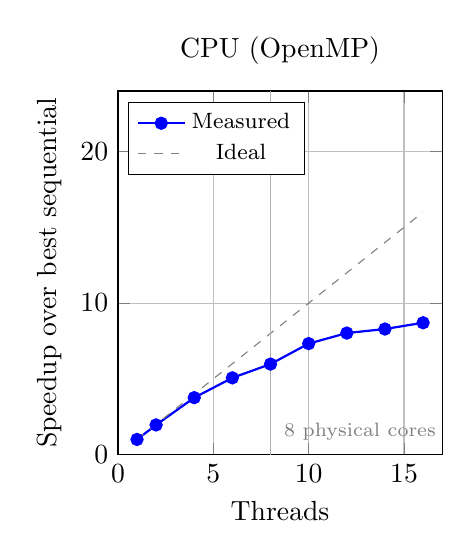
\begin{tikzpicture}
\begin{axis}[
    width=0.47\textwidth, height=6.2cm,
    title={CPU (OpenMP)}, xlabel={Threads}, ylabel={Speedup over best sequential},
    xmin=0, xmax=17, ymin=0, ymax=24, grid=major, legend pos=north west,
    legend style={font=\footnotesize}]
    \addplot[blue, mark=*, thick] coordinates {(1,1.000) (2,1.959) (4,3.758) (6,5.066) (8,5.973)
        (10,7.326) (12,8.021) (14,8.288) (16,8.701)};
    \addlegendentry{Measured}
    \addplot[dashed, gray, domain=1:16] {x};
    \addlegendentry{Ideal}
    \draw[gray!60] (axis cs:8,0) -- (axis cs:8,24);
    \node[font=\scriptsize, anchor=south west, gray] at (axis cs:8.2,0.3) {8 physical cores};
\end{axis}
\end{tikzpicture}\hfill
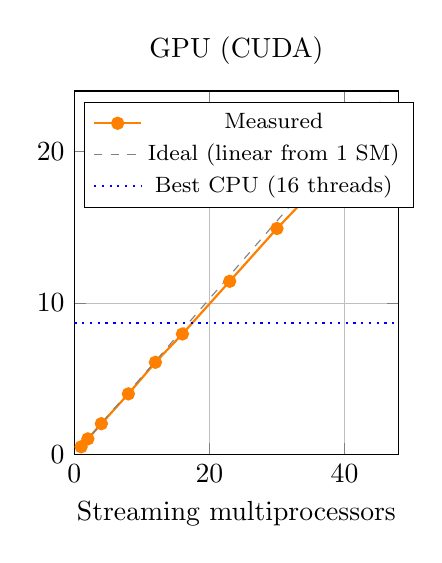
\begin{tikzpicture}
\begin{axis}[
    width=0.47\textwidth, height=6.2cm,
    title={GPU (CUDA)}, xlabel={Streaming multiprocessors},
    xmin=0, xmax=48, ymin=0, ymax=24, grid=major, legend pos=north west,
    legend style={font=\footnotesize}]
    \addplot[orange, mark=*, thick] coordinates {(1,0.514) (2,1.038) (4,2.040) (8,4.008)
        (12,6.091) (16,7.960) (23,11.437) (30,14.923) (38,18.641) (46,22.289)};
    \addlegendentry{Measured}
    \addplot[dashed, gray, domain=1:46] {0.514*x};
    \addlegendentry{Ideal (linear from 1 SM)}
    \addplot[blue, dotted, thick, domain=0:48] {8.701};
    \addlegendentry{Best CPU (16 threads)}
\end{axis}
\end{tikzpicture}
\caption{Strong scaling, whole brain. Speedup relative to the best sequential version on one CPU
core (5.24\,s, median of five runs). Data: \texttt{scaling/scaling.csv}.}
\label{fig:speedup}
\end{figure}

\paragraph{CPU.} Scaling is almost linear to 4 threads (94\% efficiency) and reaches 5.97$\times$
on 8 threads (75\%). The loss is mostly frequency: the Ryzen boosts one busy core far higher than
eight. Simultaneous multithreading adds a further 46\% from 8 to 16 threads (8.7$\times$), as
two threads per core hide some of each other's FP64 latency.

\paragraph{GPU.} Scaling is almost perfectly linear in SMs: 46 SMs are 43.3$\times$ faster than
one (94\% efficiency), and 22.3$\times$ faster than one CPU core. The GPU overtakes the whole
CPU at about 17 SMs.

\paragraph{Profile after parallelisation.} In the best sequential version gprof attributes 81\%
of the time to \texttt{ml\_device::ml} (63 calls per voxel): the hotspot remains the
Mittag-Leffler evaluation, now 17$\times$ cheaper and called 15$\times$ less often. The GPU
profile is summarised in Table~\ref{tab:ncu}.

\begin{table}[htbp]
\centering
\begin{tabular}{ll}
\toprule
Metric (Nsight Compute, whole brain) & Value \\
\midrule
Kernel duration & 263\,ms (under profiler) \\
Compute (SM) throughput / memory throughput & 82.4\% / 0.76\% of peak \\
Busiest pipeline & FP64, 82.4\% \\
Registers per thread & 200 \\
Theoretical / achieved occupancy & 16.7\% / 13.9\% (limited by registers) \\
Branch efficiency & 99.87\% \\
Register spills & 0 \\
\bottomrule
\end{tabular}
\caption{CUDA kernel profile.}
\label{tab:ncu}
\end{table}

\subsection{Verifying Correctness}
\label{sec:verify}

Every version writes its parameter maps as NIfTI volumes, and \texttt{compare/compare\_results.py}
compares them voxel by voxel in double precision (Table~\ref{tab:verify}).

\begin{table}[htbp]
\centering
\begin{tabular}{lrrrr}
\toprule
Comparison (180,722 voxels) & $D$ & $\beta$ & RMSE & Bit-identical \\
\midrule
C++ serial (Ceres) vs MATLAB & 98.3\% & 93.3\% & 98.6\% & 0\% \\
Best sequential vs MATLAB & 99.3\% & 98.6\% & 99.9\% & 0\% \\
OpenMP (16 threads) vs best sequential & 100\% & 100\% & 100\% & \textbf{100\%} \\
CUDA vs best sequential & 100\% & 100\% & 100\% & 7--26\% \\
\bottomrule
\end{tabular}
\caption{Fraction of voxels within tolerance ($D$ within 1\%, $\beta$ within 0.01, RMSE within 1\%).}
\label{tab:verify}
\end{table}

\begin{figure}[tbp]
\centering
\begin{minipage}[c]{0.53\textwidth}
    \centering
    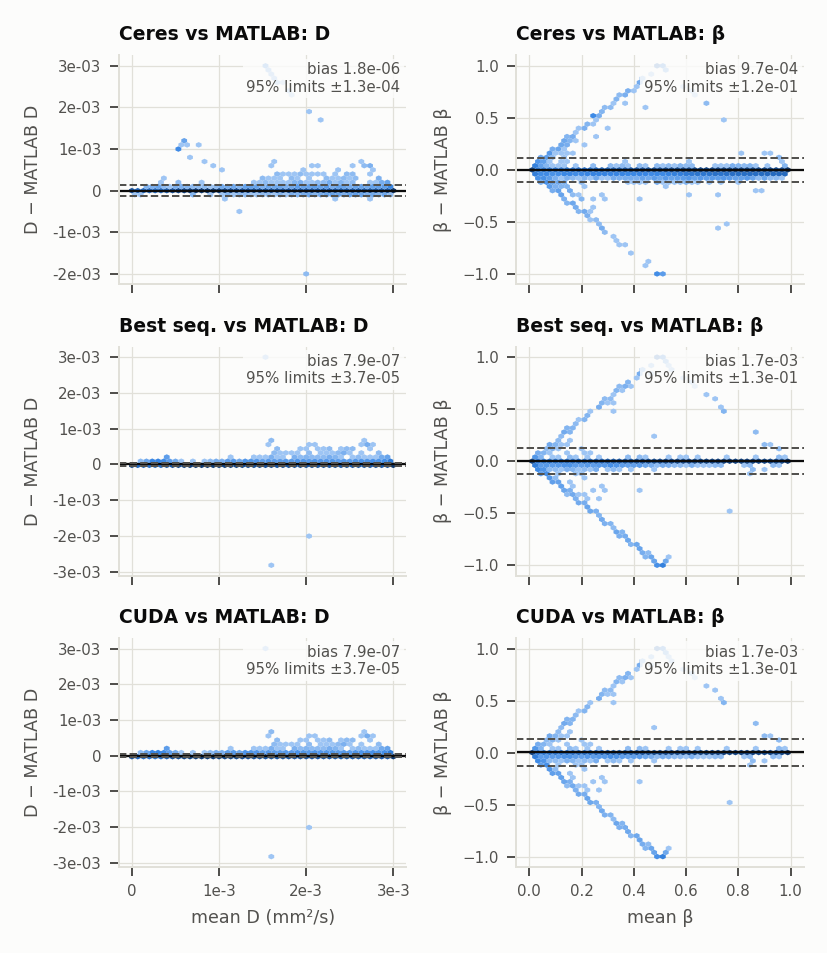
\includegraphics[width=\linewidth]{compare/all/bland_altman.png}
\end{minipage}\hfill
\begin{minipage}[c]{0.43\textwidth}
    \caption{Bland-Altman agreement with the original MATLAB fit, whole brain (180,722 voxels):
    difference against mean for $D$ (left column) and $\beta$ (right column), for the Ceres port,
    the best sequential version and CUDA. Solid line: bias; dashed: 95\% limits of agreement.
    Almost all voxels lie in the thin band at zero. The diagonal lines are voxels where one
    method placed $\beta$ (or $D$) on a bound: if one value is 0, the point must lie on
    difference $= \pm 2 \times$ mean, and if one is 1, on difference $= \pm(2 - 2 \times$ mean$)$.
    These are poorly determined voxels (see text).}
    \label{fig:ba}
\end{minipage}
\end{figure}

\textbf{OpenMP produces exactly the same results as the sequential version}: all 180,722
voxels are bit-identical for any thread count, because each voxel's fit is independent and
deterministic.

\textbf{CUDA differs from the sequential version only by floating-point rounding}: at most
$5.7\times10^{-13}$ in $D$ and $3.6\times10^{-9}$ in $\beta$. The GPU evaluates \texttt{sincos}
and fused multiply-adds slightly differently; in a few voxels this changes when the solver
stops, giving the larger maxima.

\textbf{Against the original MATLAB} no C++ version can be bit-identical (different solvers
stopping at a tolerance of $10^{-5}$), so agreement is measured. The best sequential (and so the
parallel) versions agree with MATLAB more closely than the direct Ceres port, and their fit is
more than 1\% worse than MATLAB's in only 134 voxels (0.07\%), against 2,469 (1.37\%) for Ceres.

\textbf{The remaining disagreements} (Figure~\ref{fig:ba}) are poorly determined voxels: 84\% of
voxels with $|\Delta\beta| > 0.1$ have $\beta$ on a bound in one method, 64\% have $D \approx 0$
(where $E_\beta(0) = 1$ for every $\beta$, so $\beta$ is unidentifiable), 82\% lie on the edge of
the brain mask, and their median RMSE is 1.12 against 0.016 overall. Both methods fit them
equally well (RMSE within 1\% in 87\%).

Component tests also support correctness: the NIfTI reader is bit-identical to MATLAB's
\texttt{niftiread}, the C++ Mittag-Leffler port matches \texttt{ml.m} to $6.2\times10^{-16}$, and
the device version matches the C++ port to $8.9\times10^{-16}$.

\begin{figure}[htbp]
\centering
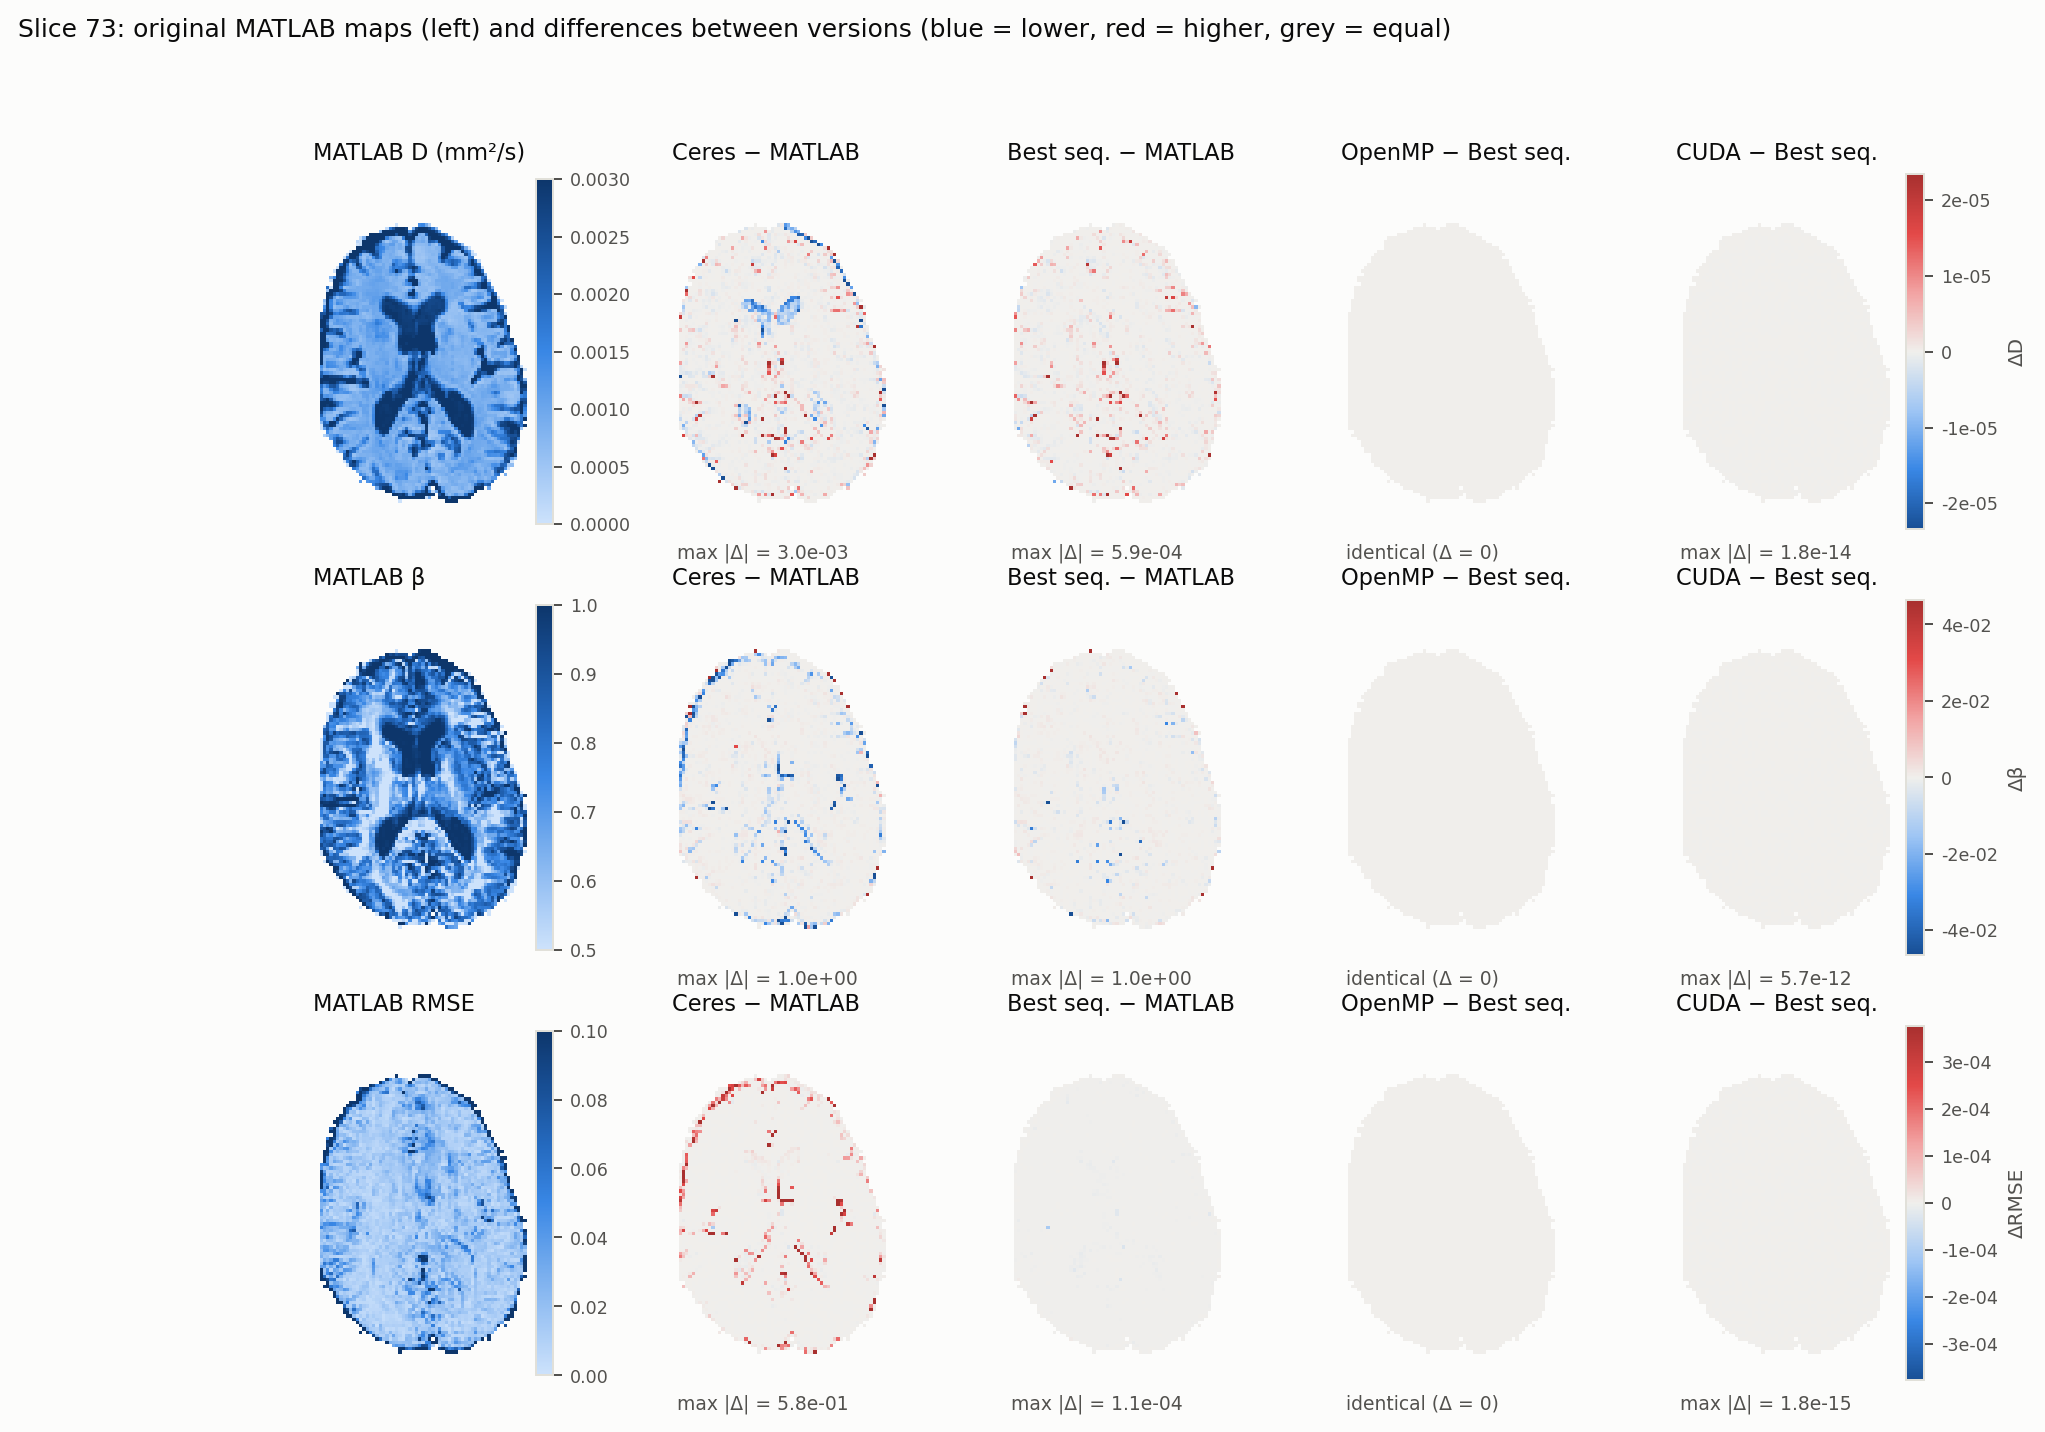
\includegraphics[width=0.88\textwidth]{compare/slice_73/maps_slice_73.png}
\caption{Slice 73. Left: original MATLAB maps. Right: differences between versions (blue lower,
red higher, grey equal). OpenMP and CUDA are indistinguishable from the best sequential version.}
\label{fig:maps}
\end{figure}

% =====================================================================
\section{Summary of Code Changes}

\begin{table}[htbp]
\centering
\begin{tabular}{lrr}
\toprule
Component & Lines & Code lines \\
\midrule
Original MATLAB (\texttt{fit\_dMRI\_signals\_19.m}, \texttt{fit\_voxel\_sub\_ml.m}, \texttt{ml.m}) & 474 & 303 \\
C++ serial port (reader, \texttt{ml} port, Ceres fit, PNG output, main, CMake) & 1,060 & 788 \\
Parallel algorithm shared by CPU and GPU (\texttt{*.cuh}) & 324 & 231 \\
CUDA host code and kernels (\texttt{main.cu}, CMake, error checking) & 508 & 414 \\
CUDA tests (\texttt{test\_ml.cu}, \texttt{compare\_serial.cu}) & 308 & 246 \\
OpenMP changes in \texttt{main.cpp} (pragma, flattened loop, \texttt{--threads}) & $\approx$60 & $\approx$45 \\
Analysis and benchmarking scripts (MATLAB, Python) & 574 & 476 \\
\bottomrule
\end{tabular}
\caption{Size of each component (code lines exclude blank lines and comments).}
\end{table}

\begin{itemize}
    \item \textbf{Specialised Mittag-Leffler function} (\texttt{mittag-leffler.cuh}): fixed contour,
        precomputed node tables, analytic derivatives, host/device compilation.
    \item \textbf{Bounded Levenberg-Marquardt solver} (\texttt{fit\_voxel\_sub\_ml.cuh}): replaces Ceres.
    \item \textbf{OpenMP}: flattened voxel loop with dynamic scheduling; \texttt{--threads} option;
        \texttt{fit\_sub\_best} build target.
    \item \textbf{CUDA}: voxel packing, constant-memory tables, one-thread-per-voxel kernel,
        SM-limited kernel with an atomic work queue, warm-up launch, \texttt{--sms} option.
    \item \textbf{Output and verification}: NIfTI output of every map, run metadata, the comparison
        and scaling scripts.
\end{itemize}

% =====================================================================
\section{Reflection}
\label{sec:reflection}

\paragraph{What was learnt.} The largest gain did not come from parallel hardware but from
understanding the computation: profiling showed that almost all the time was a special function
evaluated hundreds of times per voxel through general-purpose code, and analysing that code for
the inputs actually used reduced it to a fixed quadrature. That restructuring was also what made
the GPU possible at all. A second lesson was that measurements are easy to get wrong: debug
builds, lazy loading, concurrent benchmarks and baselines that mix algorithmic and parallel gains
all produced misleading numbers at some point.

\paragraph{How successful.} The parallel versions scale well: 94\% efficiency across 46 GPU SMs,
and on the CPU near-linear scaling until frequency effects set in. Results are bit-identical
(OpenMP) or identical to rounding (CUDA) with the sequential version, and closer to the original
MATLAB than the direct port. End to end, a 13-minute analysis now takes a quarter of a second.

\paragraph{Could it be better?} Probably, by about 2--4$\times$ more. The GPU profile shows the FP64
pipeline is the bottleneck, and the code does redundant FP64 work: each solver iteration calls
\texttt{ml(z, $\beta$)} for nine b-values with the same $\beta$, and each call recomputes
\texttt{exp} and \texttt{sincos} at all 28 nodes although they depend only on $\beta$. Hoisting them
out would cut that work about ninefold on both CPU and GPU. Single precision could be much faster
again on this GPU, if an accuracy study showed it acceptable. Higher occupancy would add little
while the FP64 units are saturated.

\paragraph{What I would do differently.} Profile the original and plan the baseline first: the
first CUDA timings were compared against the Ceres port, and only later separated into
algorithmic and parallel speedups. I would also build the comparison tooling (NIfTI outputs,
difference maps) at the start rather than checking results with images, and run benchmarks
strictly one at a time from the beginning.

\begin{thebibliography}{9}
\bibitem{garrappa2015} R.~Garrappa, \emph{Numerical evaluation of two and three parameter
    Mittag-Leffler functions}, SIAM Journal on Numerical Analysis 53(3), 1350--1369, 2015.
\bibitem{ceres} S.~Agarwal, K.~Mierle and The Ceres Solver Team, \emph{Ceres Solver},
    \url{http://ceres-solver.org}, version 2.2, 2023.
\bibitem{cuda} NVIDIA, \emph{CUDA C++ Programming Guide} and \emph{Nsight Compute Profiling Guide},
    version 13.4, 2026.
\end{thebibliography}

\newpage
\appendix

\section{Build and Run Instructions}

Source code: \textit{[TODO: repository / OneDrive link]}. Full commands are in \texttt{RESULTS.md}
and \texttt{profiling/README.md}; run everything from the repository root.

\paragraph{Serial, best sequential and OpenMP} (MSYS2 UCRT64 g++ with Ceres, Eigen and Ninja):
\begin{lstlisting}[numbers=none]
pacman -S mingw-w64-ucrt-x86_64-ceres-solver mingw-w64-ucrt-x86_64-eigen3 mingw-w64-ucrt-x86_64-ninja
cmake -S serial_cpp -B serial_cpp/build -G Ninja -DCMAKE_CXX_COMPILER=C:/msys64/ucrt64/bin/g++.exe -DCMAKE_PREFIX_PATH=C:/msys64/ucrt64
cmake --build serial_cpp/build
serial_cpp/build/fit_sub.exe --all                 # C++ serial (Ceres)
serial_cpp/build/fit_sub_best.exe --all            # best sequential
serial_cpp/build/fit_sub_best.exe --all --threads 16
\end{lstlisting}

\paragraph{CUDA} (CUDA Toolkit 13.4, Visual Studio 2026; from an x64 Visual Studio shell):
\begin{lstlisting}[numbers=none]
cmake -S cuda -B cuda/build -G Ninja
cmake --build cuda/build
cuda/build/test_ml.exe
cuda/build/fit_sub_cuda.exe --all                  # --sms N limits the SMs used
\end{lstlisting}

\paragraph{MATLAB, comparison and scaling:}
\begin{lstlisting}[numbers=none]
matlab -batch "addpath('MATLAB'); run_fit()"
python compare/compare_results.py --run all
python scaling/run_scaling.py
\end{lstlisting}
All programs accept \texttt{--slice N} to fit one axial slice.

\section{Hardware Used}

\begin{tabular}{ll}
CPU & AMD Ryzen 7 7700, 8 cores / 16 threads, 3.8\,GHz base \\
Memory & 32\,GB DDR5-4800 \\
GPU & NVIDIA GeForce RTX 4070, 46 SMs, 12\,GB, compute capability 8.9 \\
GPU driver & 617.42 \\
OS & Windows 11 Home \\
\end{tabular}

\section{Input Data Sets}

One subject (\texttt{sub\_001}) of in-vivo human brain diffusion MRI
\textit{[TODO: source, e.g. provided by supervisor / public dataset name and licence]}.
The folder \texttt{data/dwi\_real/} holds a brain mask (\texttt{*\_brainmask.nii.gz}), the $b=0$ image, and
direction-averaged images for $\Delta = 19$\,ms ($b = 50$--$6000$\,s/mm$^2$, used here) and
$\Delta = 49$\,ms; plus the full 4D series (850 volumes: 32--64 gradient directions per b-value).
The fit uses 180,722 brain voxels of the $66 \times 108 \times 108$ volume. The data are not in
the repository and must be placed in \texttt{data/dwi\_real/}.

\end{document}
